\section{Testes A/B e Permutação}

\begin{frame}{Testes A/B e a Lógica de Permutação}
    \begin{block}{A Lógica da Permutação de Rótulos}
        Se a hipótese nula $H_0$ é verdadeira (não há diferença entre o grupo de Tratamento e Controle), a associação entre as variáveis é irrelevante. Logo, podemos embaralhar aleatoriamente os rótulos dos grupos sem alterar a estrutura básica dos dados.
    \end{block}
    \begin{block}{Algoritmo Geral:}
        \begin{enumerate}
            \item Reúna os dados dos dois grupos em um único vetor.
            \item Embaralhe aleatoriamente os elementos.
            \item Separe a primeira amostra com tamanho $N_A$ (grupo A) e a segunda com $N_B$ (grupo B).
            \item Calcule a diferença de médias.
            \item Repita o processo $10.000$ vezes para criar a distribuição nula.
        \end{enumerate}
    \end{block}
\end{frame}

\begin{frame}{Caso 1: Tabagismo Materno e Peso do Bebê}
    \begin{block}{Pergunta Científica}
        O tabagismo de gestantes afeta o peso do recém-nascido?
    \end{block}
    \begin{columns}
        \begin{column}{0.5\textwidth}
            \textbf{Detalhes dos Grupos:}
            \begin{itemize}
                \item Grupo A (Fumantes): $459$ bebês.
                \item Grupo B (Não Fumantes): $715$ bebês.
                \item Estatística: $\bar{X}_B - \bar{X}_A$
                \item Diferença de médias observada: $0.26$ kg.
            \end{itemize}
        \end{column}
        \begin{column}{0.5\textwidth}
            \centering
            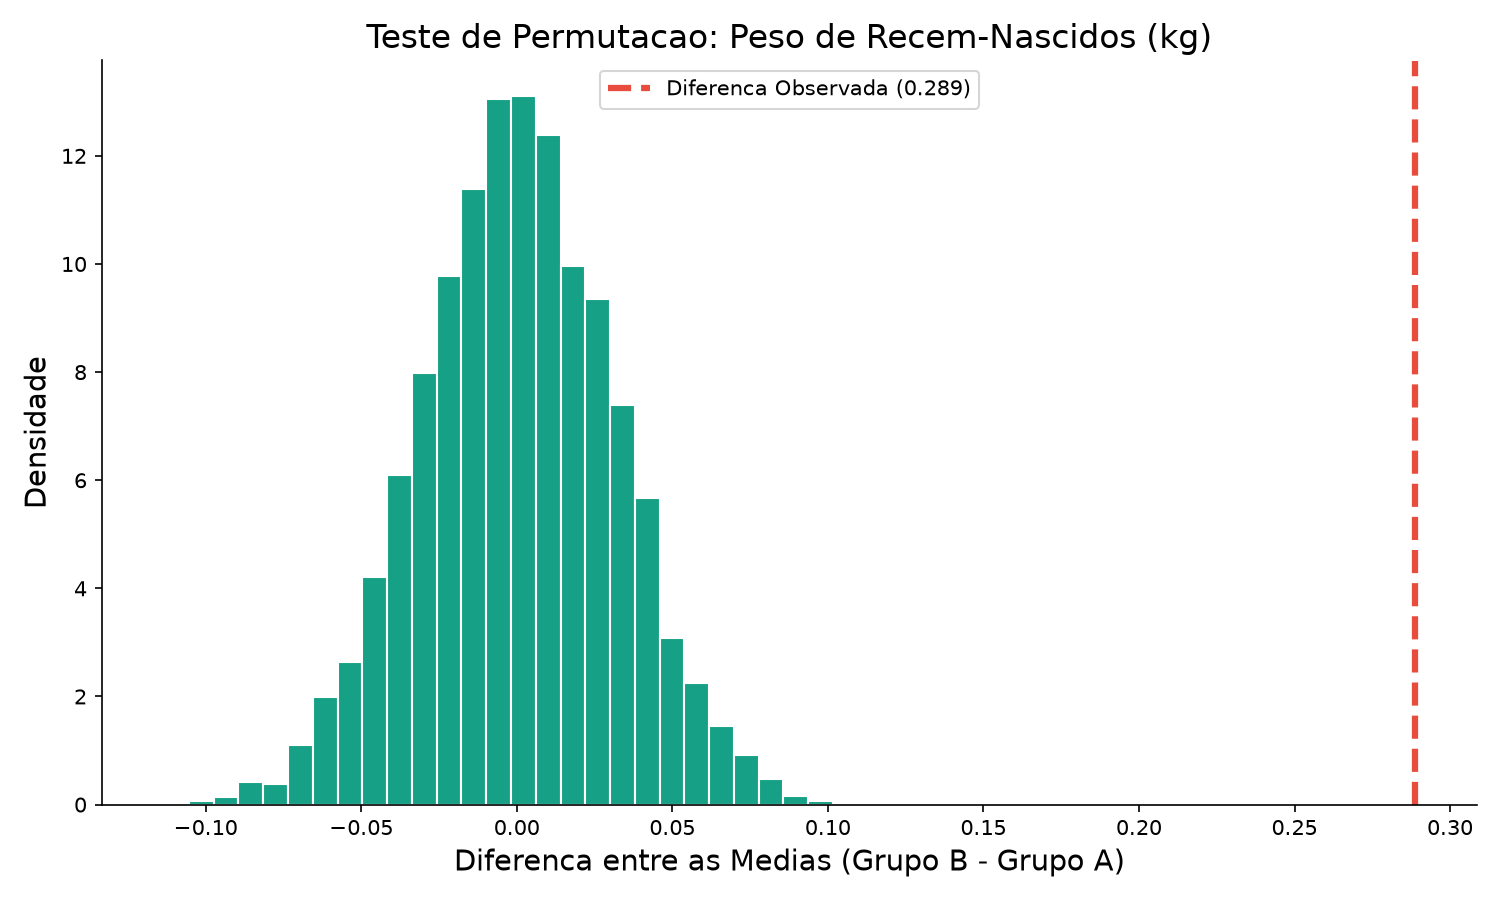
\includegraphics[width=\textwidth]{04_permutacao_peso.png}
        \end{column}
    \end{columns}
\end{frame}

\begin{frame}[fragile]{Código em Python: Permutação de Peso de Bebês}
\begin{lstlisting}[language=Python]
import numpy as np

conjunto = np.concatenate([grupo_fumantes, grupo_nao_fumantes])
n_a = len(grupo_fumantes)
diferencas = []
np.random.seed(42)

for _ in range(10000):
    # Embaralha os pesos de todos os bebes
    embaralhado = np.random.permutation(conjunto)
    sim_a = embaralhado[:n_a]
    sim_b = embaralhado[n_a:]
    diferencas.append(np.mean(sim_b) - np.mean(sim_a))

# Calcula o P-valor
p_valor = np.count_nonzero(diferencas >= 0.26) / 10000
print(f"P-valor: {p_valor:.4f}")
# Saida: 0.0000
\end{lstlisting}
\end{frame}

\begin{frame}{Simulação no Modelo Nulo e Caudas do Teste}
    \begin{block}{O que significa ``ser mais extremo''?}
        Dependendo de como definimos a nossa \textbf{Hipótese Alternativa ($H_1$)}, medimos o desvio em caudas diferentes da distribuição:
        \begin{enumerate}
            \item \textbf{Unilateral (Cauda Direita):} $\text{Média}_{\text{Não-Fumante}} > \text{Média}_{\text{Fumante}}$
            \begin{itemize}
                \item Buscamos proporção de valores simulados $\geq 0.26$ kg.
            \end{itemize}
            \item \textbf{Unilateral (Cauda Esquerda):} $\text{Média}_{\text{Não-Fumante}} < \text{Média}_{\text{Fumante}}$
            \begin{itemize}
                \item Buscamos proporção de valores simulados $\leq 0.26$ kg.
            \end{itemize}
            \item \textbf{Bicaudal (Duas Caudas):} $\text{Média}_{\text{Não-Fumante}} \neq \text{Média}_{\text{Fumante}}$
            \begin{itemize}
                \item Buscamos proporção de valores em módulo $|\text{simulado}| \geq 0.26$ kg.
            \end{itemize}
        \end{enumerate}
    \end{block}
    \centering
    \textit{Cada alternativa altera a área (cauda) que calculamos para obter o P-valor.}
\end{frame}

\begin{frame}{Decisão Estatística: Peso de Bebês}
    \begin{block}{Resultado Obtido}
        \begin{itemize}
            \item Diferença de médias observada na amostra real: $0.26$ kg.
            \item Em $10.000$ embaralhamentos (permutações) simulados sob a hipótese nula $H_0$, a diferença de médias nunca alcançou $0.26$ kg.
            \item Nosso $p$-valor empírico foi de $0.0000$ ($0\%$).
        \end{itemize}
    \end{block}
    \begin{alertblock}{Tomada de Decisão}
        Como $p$-valor ($0\%$) $<$ Limiar de Significância ($\alpha = 5\%$), \textbf{rejeitamos a hipótese nula $H_0$}.
    \end{alertblock}
    \centering
    \textbf{Conclusão:} O tabagismo na gestação está estatisticamente associado a uma redução sistemática no peso do recém-nascido. A diferença não é explicável pelo acaso.
\end{frame}

\begin{frame}{Caso 2: Salários NBA (Cleveland vs. Houston)}
    \begin{block}{O Problema de Variância}
        Cleveland Cavs e Houston Rockets têm salários médios aparentando diferença ($10.23$ M\$ vs $7.10$ M\$ na população). Porém, a variância de salários na NBA é extremamente alta e a amostra de jogadores disponível é muito pequena ($N = 15$ por time).
    \end{block}
    \begin{block}{Amostra Simulada ($N=15$)}
        Para ilustrar o teste computacionalmente, geramos uma amostra sintética de $15$ jogadores por time:
        \begin{itemize}
            \item Média Cleveland na Amostra: $10.34$ M\$
            \item Média Houston na Amostra: $2.85$ M\$
            \item Diferença Observada na Amostra: $7.50$ M\$
        \end{itemize}
    \end{block}
    \centering
    \textit{Será que uma diferença aparente de $7.50$ M\$ é significativa ou pode ser explicada apenas pela variabilidade natural dos salários?}
\end{frame}

\begin{frame}{Resultados de Permutações nos Salários}
    \begin{block}{Médias de Cleveland e Houston após o Shuffle}
        Sob a hipótese nula $H_0$, a designação do time é mero rótulo. Ao misturar todos os salários e sorteá-los em dois grupos de 15, veja como as médias variam por puro acaso:
    \end{block}
    
    \begin{table}
        \centering
        \small
        \begin{tabular}{lccc}
            \toprule
            \textbf{Rodada (Shuffle)} & \textbf{Média Cleveland} & \textbf{Média Houston} & \textbf{Diferença ($C - H$)} \\
            \midrule
            Amostra Real Simulada & $10.34$ M\$ & $2.85$ M\$ & $7.50$ M\$ \\
            \midrule
            Simulação 1 & $7.92$ M\$ & $5.27$ M\$ & $2.64$ M\$ \\
            Simulação 2 & $4.79$ M\$ & $8.40$ M\$ & $-3.61$ M\$ \\
            Simulação 3 & $9.13$ M\$ & $4.06$ M\$ & $5.08$ M\$ \\
            Simulação 4 & $5.23$ M\$ & $7.96$ M\$ & $-2.74$ M\$ \\
            \bottomrule
        \end{tabular}
        \caption{Exemplos de médias e diferenças após permutações}
    \end{table}
    \centering
    \textit{Note que mesmo no modelo nulo (sem efeito real), as diferenças flutuam bastante devido à alta variabilidade dos dados.}
\end{frame}

\begin{frame}[fragile]{Código em Python: Salários da NBA}
\begin{lstlisting}[language=Python]
import numpy as np

conjunto = np.concatenate([grupo_houston, grupo_cleveland])
n_a = len(grupo_houston)
diferencas_nba = []
np.random.seed(42)

for _ in range(10000):
    # Embaralha os salarios dos jogadores
    embaralhado = np.random.permutation(conjunto)
    sim_a = embaralhado[:n_a]
    sim_b = embaralhado[n_a:]
    diferencas_nba.append(np.mean(sim_b) - np.mean(sim_a))

# Teste bicaudal para o P-valor
obs_diff = 7.50
p_valor = np.count_nonzero(np.abs(diferencas_nba) >= np.abs(obs_diff)) / 10000
print(f"P-valor bicaudal: {p_valor:.4f}")
# Saida: 0.1010
\end{lstlisting}
\end{frame}

\begin{frame}{Decisão Estatística: Salários da NBA}
    \begin{columns}
        \begin{column}{0.5\textwidth}
            \textbf{Análise do P-valor Bicaudal:}
            \begin{itemize}
                \item Diferença de médias na amostra: $7.50$ M\$.
                \item P-valor bicaudal: $10.10\%$.
                \item Como $p\text{-valor} \geq 5\%$, \textbf{não rejeitamos a hipótese nula $H_0$}.
            \end{itemize}
            \vspace{0.2cm}
            \textbf{Conclusão:} A diferença observada nos salários não é estatisticamente significante; a alta variação salarial combinada com a amostra pequena torna a diferença explicável pelo acaso.
        \end{column}
        \begin{column}{0.5\textwidth}
            \centering
            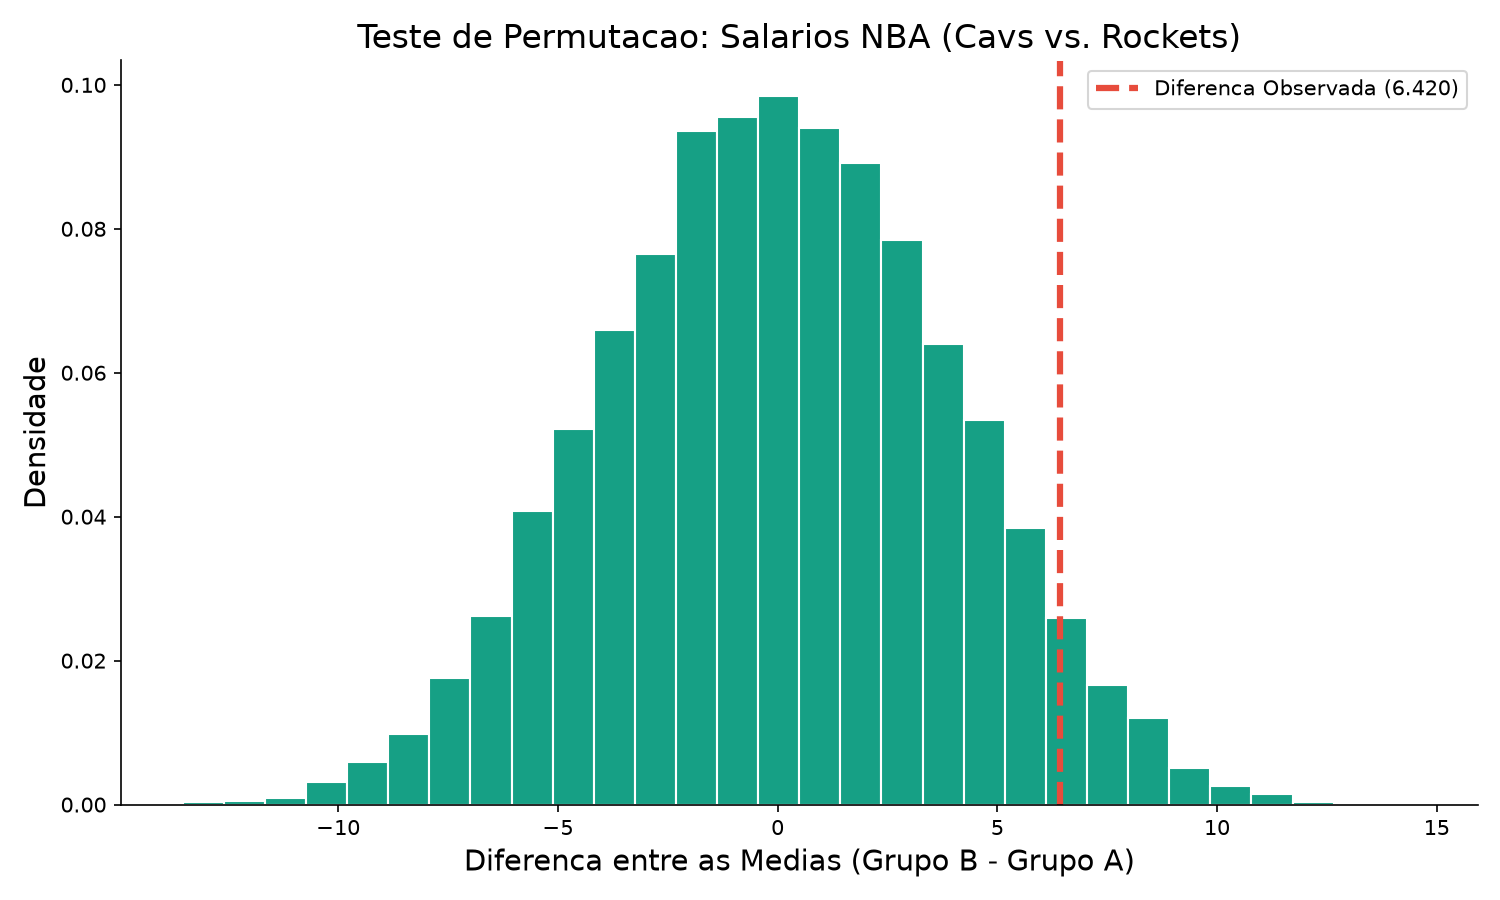
\includegraphics[width=\textwidth]{05_permutacao_nba.png}
        \end{column}
    \end{columns}
\end{frame}
